\documentclass{standalone}
\usepackage{tikz}
\usetikzlibrary{patterns, positioning}
\usepackage[sfdefault]{ClearSans} %% option 'sfdefault' activates Clear Sans as the default text font
\usepackage[T1]{fontenc}

\begin{document}
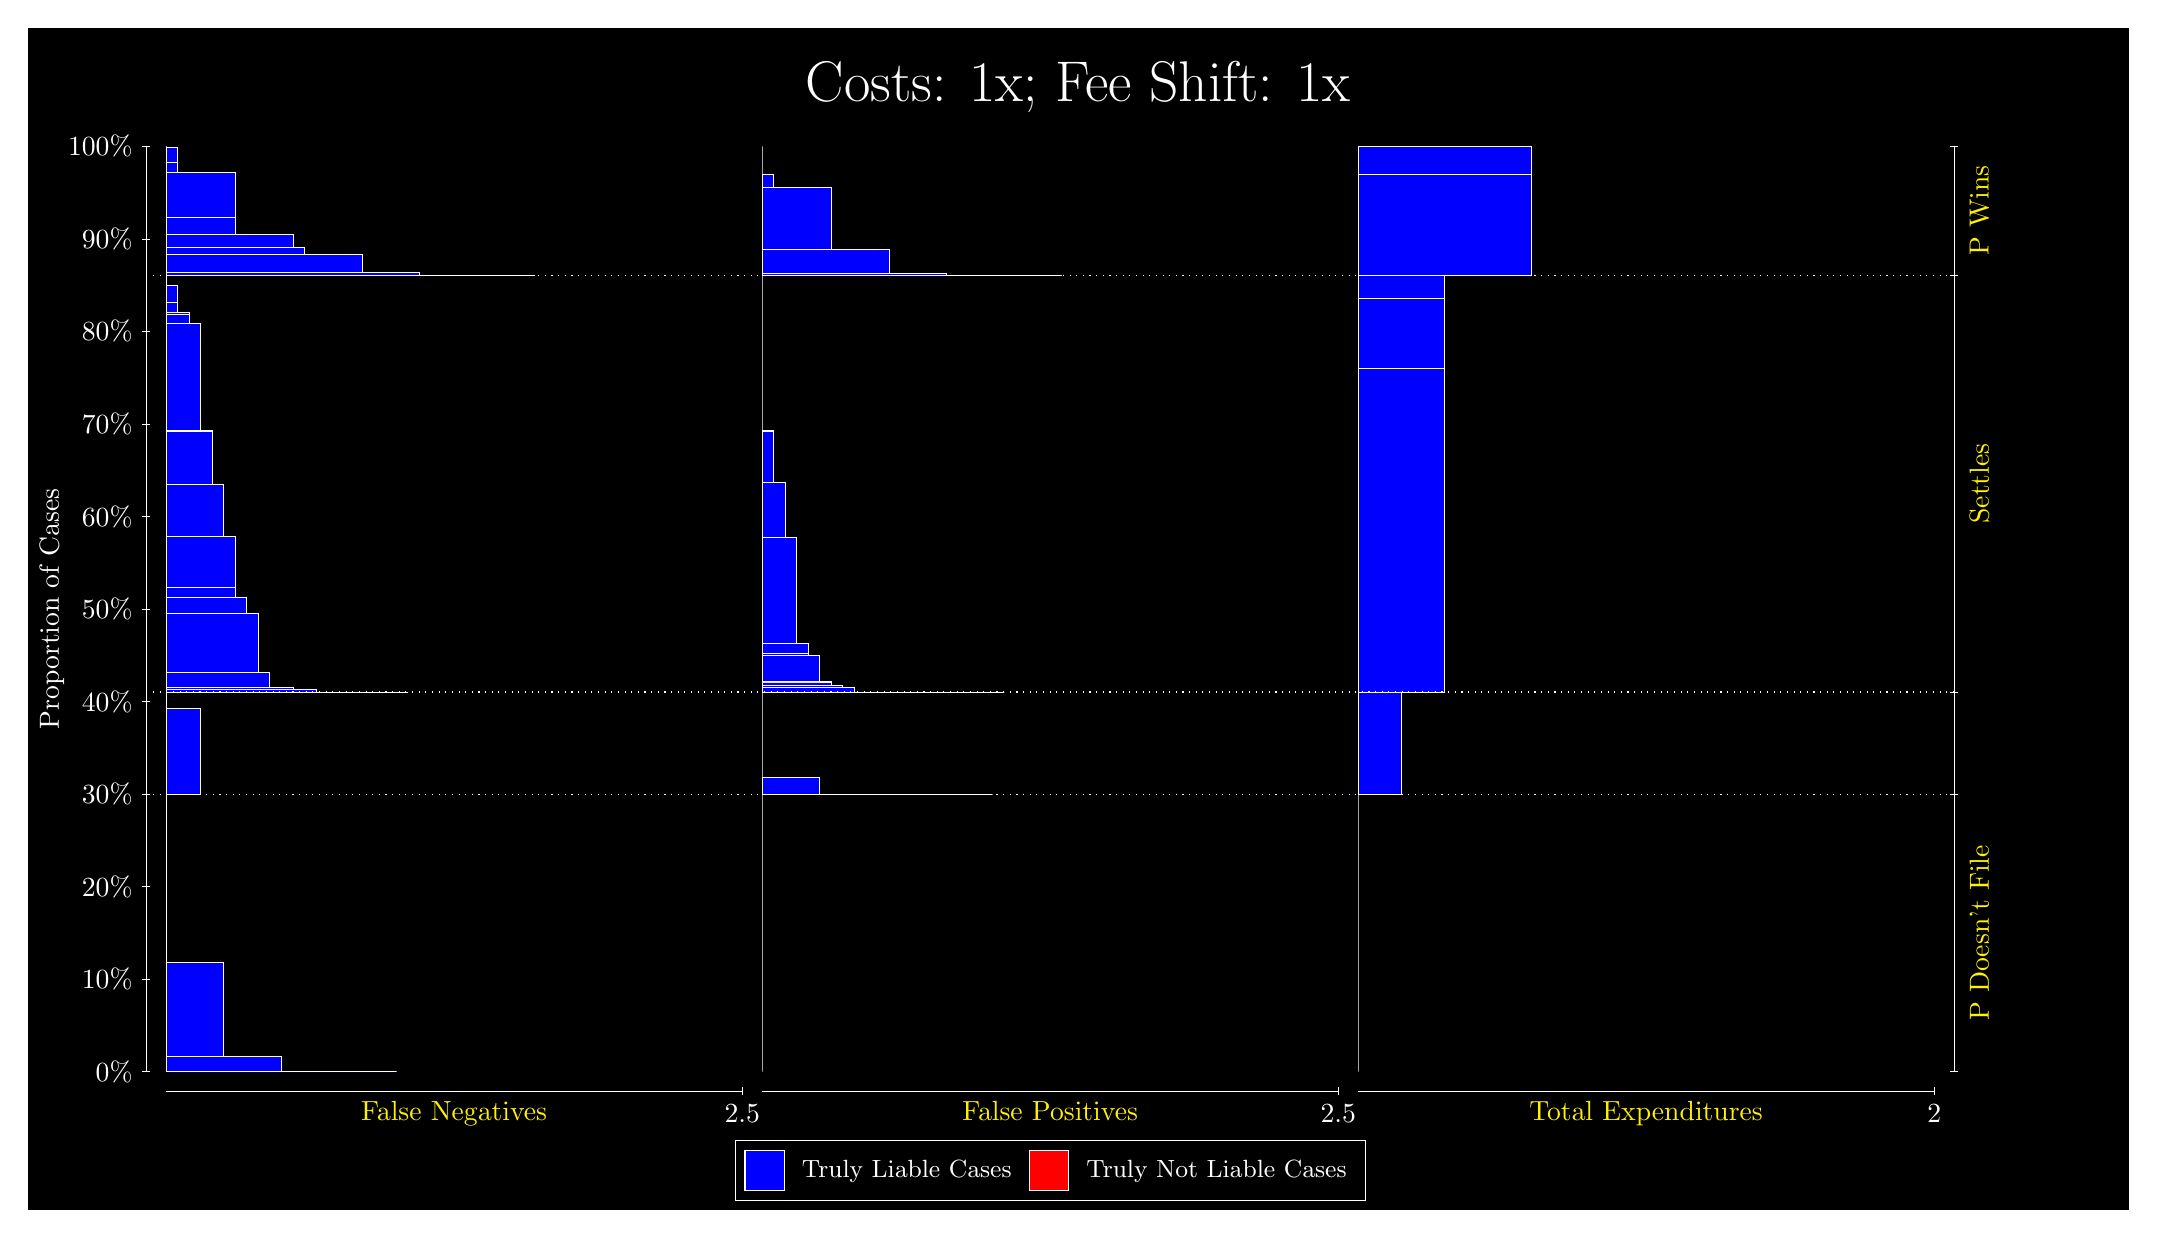
\begin{tikzpicture}
\draw[fill=black] (0,0) rectangle (26.667,15);
\draw[text=white] (0,13.5) rectangle (26.667,15) node[midway] {\huge Costs: 1x; Fee Shift: 1x};
\draw[white, very thin] (1.5,1.75) -- (1.5,13.5);
\node[rotate=90, text=white, anchor=center] at (0.3, 7.625) {Proportion of Cases};
\draw[white, very thin] (1.45,1.75) -- (1.55,1.75);
\node[text=white, anchor=east] at (1.45, 1.75) {0\%};
\draw[white, very thin] (1.45,2.925) -- (1.55,2.925);
\node[text=white, anchor=east] at (1.45, 2.925) {10\%};
\draw[white, very thin] (1.45,4.1) -- (1.55,4.1);
\node[text=white, anchor=east] at (1.45, 4.1) {20\%};
\draw[white, very thin] (1.45,5.275) -- (1.55,5.275);
\node[text=white, anchor=east] at (1.45, 5.275) {30\%};
\draw[white, very thin] (1.45,6.45) -- (1.55,6.45);
\node[text=white, anchor=east] at (1.45, 6.45) {40\%};
\draw[white, very thin] (1.45,7.625) -- (1.55,7.625);
\node[text=white, anchor=east] at (1.45, 7.625) {50\%};
\draw[white, very thin] (1.45,8.8) -- (1.55,8.8);
\node[text=white, anchor=east] at (1.45, 8.8) {60\%};
\draw[white, very thin] (1.45,9.975) -- (1.55,9.975);
\node[text=white, anchor=east] at (1.45, 9.975) {70\%};
\draw[white, very thin] (1.45,11.15) -- (1.55,11.15);
\node[text=white, anchor=east] at (1.45, 11.15) {80\%};
\draw[white, very thin] (1.45,12.325) -- (1.55,12.325);
\node[text=white, anchor=east] at (1.45, 12.325) {90\%};
\draw[white, very thin] (1.45,13.5) -- (1.55,13.5);
\node[text=white, anchor=east] at (1.45, 13.5) {100\%};

\draw[white, very thin] (24.457,1.75) -- (24.457,13.5);
\draw[white, very thin] (24.407,1.75) -- (24.507,1.75);
\node[anchor=west] at (24.407, 1.75) {};
\draw[white, very thin] (24.407,5.2709) -- (24.507,5.2709);
\node[anchor=west] at (24.407, 5.2709) {};
\draw[white, very thin] (24.407,6.5705) -- (24.507,6.5705);
\node[anchor=west] at (24.407, 6.5705) {};
\draw[white, very thin] (24.407,11.865) -- (24.507,11.865);
\node[anchor=west] at (24.407, 11.865) {};
\draw[white, very thin] (24.407,13.5) -- (24.507,13.5);
\node[anchor=west] at (24.407, 13.5) {};

\draw[white, very thin, fill=blue] (1.75,1.75) rectangle (4.6775,1.75);
\draw[white, very thin, fill=blue] (1.75,1.75) rectangle (3.9457,1.7516);
\draw[white, very thin, fill=blue] (1.75,1.7516) rectangle (3.2138,1.9444);
\draw[white, very thin, fill=blue] (1.75,1.9444) rectangle (2.4819,3.1387);
\draw[white, very thin, fill=red] (1.75,3.1387) rectangle (1.75,3.1387);
\draw[white, very thin, fill=blue] (1.75,3.1387) rectangle (1.75,5.2709);
\draw[white, very thin, fill=blue] (1.75,5.2709) rectangle (2.1891,6.358);
\draw[white, very thin, fill=red] (1.75,6.358) rectangle (1.75,6.358);
\draw[white, very thin, fill=blue] (1.75,6.358) rectangle (1.75,6.5705);
\draw[white, very thin, fill=blue] (1.75,6.5705) rectangle (4.8239,6.5705);
\draw[white, very thin, fill=blue] (1.75,6.5705) rectangle (4.5312,6.5705);
\draw[white, very thin, fill=blue] (1.75,6.5705) rectangle (4.2384,6.5705);
\draw[white, very thin, fill=blue] (1.75,6.5705) rectangle (4.092,6.5706);
\draw[white, very thin, fill=blue] (1.75,6.5706) rectangle (3.9457,6.5706);
\draw[white, very thin, fill=blue] (1.75,6.5706) rectangle (3.7993,6.5706);
\draw[white, very thin, fill=blue] (1.75,6.5706) rectangle (3.6529,6.6052);
\draw[white, very thin, fill=blue] (1.75,6.6052) rectangle (3.5065,6.606);
\draw[white, very thin, fill=blue] (1.75,6.606) rectangle (3.3602,6.6342);
\draw[white, very thin, fill=blue] (1.75,6.6342) rectangle (3.2138,6.6347);
\draw[white, very thin, fill=blue] (1.75,6.6347) rectangle (3.0674,6.8202);
\draw[white, very thin, fill=blue] (1.75,6.8202) rectangle (3.0674,6.8209);
\draw[white, very thin, fill=blue] (1.75,6.8209) rectangle (2.921,7.5656);
\draw[white, very thin, fill=blue] (1.75,7.5656) rectangle (2.7746,7.774);
\draw[white, very thin, fill=blue] (1.75,7.774) rectangle (2.6283,7.9005);
\draw[white, very thin, fill=blue] (1.75,7.9005) rectangle (2.6283,8.5444);
\draw[white, very thin, fill=blue] (1.75,8.5444) rectangle (2.4819,9.207);
\draw[white, very thin, fill=blue] (1.75,9.207) rectangle (2.3355,9.8828);
\draw[white, very thin, fill=blue] (1.75,9.8828) rectangle (2.3355,9.897);
\draw[white, very thin, fill=blue] (1.75,9.897) rectangle (2.1891,11.247);
\draw[white, very thin, fill=blue] (1.75,11.247) rectangle (2.0428,11.371);
\draw[white, very thin, fill=blue] (1.75,11.371) rectangle (2.0428,11.397);
\draw[white, very thin, fill=blue] (1.75,11.397) rectangle (1.8964,11.523);
\draw[white, very thin, fill=blue] (1.75,11.523) rectangle (1.8964,11.735);
\draw[white, very thin, fill=blue] (1.75,11.735) rectangle (1.75,11.736);
\draw[white, very thin, fill=red] (1.75,11.736) rectangle (1.75,11.736);
\draw[white, very thin, fill=blue] (1.75,11.736) rectangle (1.75,11.865);
\draw[white, very thin, fill=blue] (1.75,11.865) rectangle (6.4341,11.865);
\draw[white, very thin, fill=blue] (1.75,11.865) rectangle (5.7022,11.865);
\draw[white, very thin, fill=blue] (1.75,11.865) rectangle (4.9703,11.897);
\draw[white, very thin, fill=blue] (1.75,11.897) rectangle (4.8239,11.897);
\draw[white, very thin, fill=blue] (1.75,11.897) rectangle (4.2384,12.132);
\draw[white, very thin, fill=blue] (1.75,12.132) rectangle (4.092,12.132);
\draw[white, very thin, fill=blue] (1.75,12.132) rectangle (3.5065,12.215);
\draw[white, very thin, fill=blue] (1.75,12.215) rectangle (3.3602,12.385);
\draw[white, very thin, fill=blue] (1.75,12.385) rectangle (2.7746,12.385);
\draw[white, very thin, fill=blue] (1.75,12.385) rectangle (2.6283,12.599);
\draw[white, very thin, fill=blue] (1.75,12.599) rectangle (2.6283,13.176);
\draw[white, very thin, fill=blue] (1.75,13.176) rectangle (2.0428,13.176);
\draw[white, very thin, fill=blue] (1.75,13.176) rectangle (1.8964,13.299);
\draw[white, very thin, fill=blue] (1.75,13.299) rectangle (1.8964,13.482);
\draw[white, very thin, fill=red] (1.75,13.482) rectangle (1.75,13.482);
\draw[white, very thin, fill=blue] (1.75,13.482) rectangle (1.75,13.5);
\draw[white, very thin, fill=red] (9.3189,1.75) rectangle (9.3189,1.75);
\draw[white, very thin, fill=blue] (9.3189,1.75) rectangle (9.3189,5.2709);
\draw[white, very thin, fill=red] (9.3189,5.2709) rectangle (12.246,5.2709);
\draw[white, very thin, fill=blue] (9.3189,5.2709) rectangle (12.246,5.2709);
\draw[white, very thin, fill=blue] (9.3189,5.2709) rectangle (11.515,5.2709);
\draw[white, very thin, fill=blue] (9.3189,5.2709) rectangle (10.783,5.2726);
\draw[white, very thin, fill=blue] (9.3189,5.2726) rectangle (10.051,5.4835);
\draw[white, very thin, fill=blue] (9.3189,5.4835) rectangle (9.3189,6.5705);
\draw[white, very thin, fill=red] (9.3189,6.5705) rectangle (12.393,6.5705);
\draw[white, very thin, fill=blue] (9.3189,6.5705) rectangle (12.393,6.5705);
\draw[white, very thin, fill=red] (9.3189,6.5705) rectangle (12.1,6.5705);
\draw[white, very thin, fill=blue] (9.3189,6.5705) rectangle (12.1,6.5705);
\draw[white, very thin, fill=red] (9.3189,6.5705) rectangle (11.807,6.5705);
\draw[white, very thin, fill=blue] (9.3189,6.5705) rectangle (11.807,6.5705);
\draw[white, very thin, fill=blue] (9.3189,6.5705) rectangle (11.661,6.5705);
\draw[white, very thin, fill=red] (9.3189,6.5705) rectangle (11.515,6.5705);
\draw[white, very thin, fill=blue] (9.3189,6.5705) rectangle (11.515,6.5705);
\draw[white, very thin, fill=blue] (9.3189,6.5705) rectangle (11.368,6.5705);
\draw[white, very thin, fill=red] (9.3189,6.5705) rectangle (11.222,6.5705);
\draw[white, very thin, fill=blue] (9.3189,6.5705) rectangle (11.222,6.5706);
\draw[white, very thin, fill=blue] (9.3189,6.5706) rectangle (11.075,6.5706);
\draw[white, very thin, fill=blue] (9.3189,6.5706) rectangle (10.929,6.5706);
\draw[white, very thin, fill=red] (9.3189,6.5706) rectangle (10.929,6.5706);
\draw[white, very thin, fill=blue] (9.3189,6.5706) rectangle (10.929,6.5706);
\draw[white, very thin, fill=blue] (9.3189,6.5706) rectangle (10.783,6.5708);
\draw[white, very thin, fill=blue] (9.3189,6.5708) rectangle (10.636,6.5709);
\draw[white, very thin, fill=red] (9.3189,6.5709) rectangle (10.636,6.5709);
\draw[white, very thin, fill=blue] (9.3189,6.5709) rectangle (10.636,6.5712);
\draw[white, very thin, fill=blue] (9.3189,6.5712) rectangle (10.49,6.63);
\draw[white, very thin, fill=red] (9.3189,6.63) rectangle (10.344,6.63);
\draw[white, very thin, fill=blue] (9.3189,6.63) rectangle (10.344,6.6613);
\draw[white, very thin, fill=blue] (9.3189,6.6613) rectangle (10.197,6.6994);
\draw[white, very thin, fill=blue] (9.3189,6.6994) rectangle (10.197,6.7);
\draw[white, very thin, fill=red] (9.3189,6.7) rectangle (10.051,6.7);
\draw[white, very thin, fill=blue] (9.3189,6.7) rectangle (10.051,7.0387);
\draw[white, very thin, fill=blue] (9.3189,7.0387) rectangle (9.9044,7.0644);
\draw[white, very thin, fill=blue] (9.3189,7.0644) rectangle (9.9044,7.1882);
\draw[white, very thin, fill=blue] (9.3189,7.1882) rectangle (9.758,8.5384);
\draw[white, very thin, fill=blue] (9.3189,8.5384) rectangle (9.6116,9.2284);
\draw[white, very thin, fill=blue] (9.3189,9.2284) rectangle (9.4652,9.8769);
\draw[white, very thin, fill=blue] (9.3189,9.8769) rectangle (9.4652,9.891);
\draw[white, very thin, fill=blue] (9.3189,9.891) rectangle (9.3189,11.865);
\draw[white, very thin, fill=red] (9.3189,11.865) rectangle (13.125,11.865);
\draw[white, very thin, fill=blue] (9.3189,11.865) rectangle (13.125,11.865);
\draw[white, very thin, fill=red] (9.3189,11.865) rectangle (12.393,11.865);
\draw[white, very thin, fill=blue] (9.3189,11.865) rectangle (12.393,11.865);
\draw[white, very thin, fill=red] (9.3189,11.865) rectangle (11.661,11.865);
\draw[white, very thin, fill=blue] (9.3189,11.865) rectangle (11.661,11.883);
\draw[white, very thin, fill=red] (9.3189,11.883) rectangle (10.929,11.883);
\draw[white, very thin, fill=blue] (9.3189,11.883) rectangle (10.929,12.189);
\draw[white, very thin, fill=red] (9.3189,12.189) rectangle (10.783,12.189);
\draw[white, very thin, fill=blue] (9.3189,12.189) rectangle (10.783,12.189);
\draw[white, very thin, fill=blue] (9.3189,12.189) rectangle (10.197,12.98);
\draw[white, very thin, fill=red] (9.3189,12.98) rectangle (10.051,12.98);
\draw[white, very thin, fill=blue] (9.3189,12.98) rectangle (10.051,12.98);
\draw[white, very thin, fill=blue] (9.3189,12.98) rectangle (9.4652,13.15);
\draw[white, very thin, fill=red] (9.3189,13.15) rectangle (9.3189,13.15);
\draw[white, very thin, fill=blue] (9.3189,13.15) rectangle (9.3189,13.5);
\draw[white, very thin, fill=red] (16.888,1.75) rectangle (16.888,1.75);
\draw[white, very thin, fill=blue] (16.888,1.75) rectangle (16.888,5.2709);
\draw[white, very thin, fill=red] (16.888,5.2709) rectangle (17.437,5.2709);
\draw[white, very thin, fill=blue] (16.888,5.2709) rectangle (17.437,6.5705);
\draw[white, very thin, fill=red] (16.888,6.5705) rectangle (17.986,6.5705);
\draw[white, very thin, fill=blue] (16.888,6.5705) rectangle (17.986,10.687);
\draw[white, very thin, fill=red] (16.888,10.687) rectangle (17.986,10.687);
\draw[white, very thin, fill=blue] (16.888,10.687) rectangle (17.986,11.572);
\draw[white, very thin, fill=red] (16.888,11.572) rectangle (17.986,11.572);
\draw[white, very thin, fill=blue] (16.888,11.572) rectangle (17.986,11.865);
\draw[white, very thin, fill=red] (16.888,11.865) rectangle (19.083,11.865);
\draw[white, very thin, fill=blue] (16.888,11.865) rectangle (19.083,13.15);
\draw[white, very thin, fill=red] (16.888,13.15) rectangle (19.083,13.15);
\draw[white, very thin, fill=blue] (16.888,13.15) rectangle (19.083,13.5);
\draw[white, dotted] (1.5,5.2709) -- (24.457,5.2709);
\draw[white, dotted] (1.5,6.5705) -- (24.457,6.5705);
\draw[white, dotted] (1.5,11.865) -- (24.457,11.865);
\draw[white, very thin] (1.75,1.5) -- (9.0689,1.5);
\node[text=yellow, anchor=north] at (5.4094, 1.5) {False Negatives};
\draw[white, very thin] (9.0689,1.45) -- (9.0689,1.55);
\node[text=white, anchor=north] at (9.0689, 1.45) {2.5};

\draw[white, very thin] (9.3189,1.5) -- (16.638,1.5);
\node[text=yellow, anchor=north] at (12.978, 1.5) {False Positives};
\draw[white, very thin] (16.638,1.45) -- (16.638,1.55);
\node[text=white, anchor=north] at (16.638, 1.45) {2.5};

\draw[white, very thin] (16.888,1.5) -- (24.207,1.5);
\node[text=yellow, anchor=north] at (20.547, 1.5) {Total Expenditures};
\draw[white, very thin] (24.207,1.45) -- (24.207,1.55);
\node[text=white, anchor=north] at (24.207, 1.45) {2};

\node[text=yellow, centered, rotate=90] at (24.777, 3.5105) {P Doesn't File};

\node[text=yellow, centered, rotate=90] at (24.777, 9.2177) {Settles};
\node[text=yellow, centered, rotate=90] at (24.777, 12.682) {P Wins};

\draw (12.978300999999998,1.5) node[draw=none] (baseCoordinate) {};
\begin{scope}[align=center]
        \matrix[scale=0.5, draw=white, below=0.5cm of baseCoordinate, nodes={draw}, column sep=0.1cm]{
            \node[rectangle, draw, minimum width=0.5cm, minimum height=0.5cm, fill=blue] {}; &
            \node[draw=none, font=\small, text=white] (B) {Truly Liable Cases}; &
            \node[rectangle, draw, minimum width=0.5cm, minimum height=0.5cm, fill=red] {}; &
            \node[draw=none, font=\small, text=white] (B) {Truly Not Liable Cases}; \\
            };
\end{scope}

\end{tikzpicture}
\end{document}